\chapter{Compiler Entwurf}
Basierend auf der theoretischen Einführung von Compilern kann nun ein Entwurf für den Source to Source Compilers erstellt werden auf dessen Basis in späteren Kapiteln eben dieser Implementiert werden soll.  Die Phasen aus dem vorherigen Kapiteln sollen in dem in dieser dieser Arbeit zu entwickelnden Übersetzers ebenfalls durchlaufen werden.  
Wie bereits in der Definition zu Compilern aufgeführt,  muss das Ziel des Compilers sein eine gleichwertige mobile Anwendung zur Verfügung zu stellen.  Im Falle dieses Compilers bedeutet dies,  dass die resultierende Flutter App sich identisch wie die ausgehende Xamarin.Forms App verhalten sollte.  Da es sich bei beiden Frameworks um große ausgereifte Open Source Projekte handelt,  hat sich um die Frameworks eine Vielzahl von Erweiterungen in Form von Plugins entwickelt.  Da es sich bei diesen Erweiterungen nicht zwangsläufig um Open-Source Projekte handelt hat der zu entwickelnde Übersetzer keinen Zugriff auf den Quelltext und kann diesen daher nicht Übersetzen.  Der Einfachheit halber soll der in dieser Arbeit entwickelte Prototyp ausschließlich Elemente die im Eigentlichen Framework Xamarin.Forms vorhanden sind sowie die Inhalte des Optional Verfügbaren Packetes Xamarin.Essentials, welches ebenfalls von Microsoft ist übersetzen. 

\section{Struktur}

Xamarin.Forms Quelltext-Dokumente lassen sich in zwei Kategorien unterteilen.  Den XAML (Extensible Application Markup Language) Dateien,  die eine Benutzeroberfläche beschreiben,  sowie den CS- Dateien welche den C\# Quelltext beinhalten.  Bei Dateien mit der Endung XAML.CS  handelt es sich um Quelltext Dokumente,  die die Logik für eine Ansicht beschreiben.  Für die Übersetzung der Anwendung hat dies eine besondere Bedeutung,  da XAML und XAML.CS Dateien zusammen eine Ansicht und ihr Verhalten definieren.  Alleinstehende .CS Dateien beschreiben die anderen Klassen der Anwendung und können unabhängig betrachtet werden.  Abbildung \ref{fig:CompilerStruktur} zeigt die Struktur des zu realisierenden Übersetzers auf einer hohen Abstraktionsebene.
\begin{figure}[!ht]
 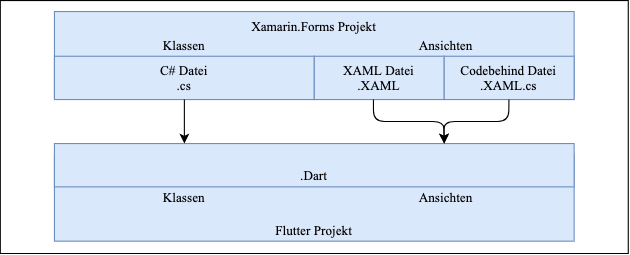
\includegraphics[width=14.5cm,height=5.3cm]{Images/Compiler/CompilerArchitecture.png}
 \caption{Compiler Struktur}
 \label{fig:}
\end{figure}

Wie man in der Abbildung sehen kann unterteilt sich die Übersetzung zwischen Dateien mit generellen Klassendefinition und jeweils zwei Dateien für Ansichten.  Für das Framework Flutter,  in welches diese Dateien überführt werden sollen gibt es nur eine Art von Dateien mit der Dateiendung Dart.
Im folgenden soll jeweils erläutert werden, wie die Dateien von Ansichten und generelle C\# Klassen übersetzt werden sollen.  Durch eine Kombination von beiden Teilen sollte anschließend eine gleichwertige mobile Anwendung ergeben. 

\subsection{Dateien für die Anzeige }
\subsection{Generelle C\# Klassen}



\section{Rosyln als Ausgangssituation}
Wichtig für den Entwurf ist die Erkenntnis,  dass der modulare C\# Compiler Roslyn als Einstiegspunkt für die Übersetzung verwendet werden kann.  So kann auf eine ausgereifte Plattform für die ersten Phasen der Compilierung zurückgegriffen werden.




\section{Code optimierung}
Die Code Optimierung ist der essentielle Teil der Übersetzung.  Beide Frameworks arbeiten grundlegend Unterschiedlich,  sodass eine einfache Übersetzung nicht zu einer funktionsfähigen Anwendung führen würde.  Daher ist es notwendig,  beide Frameworks zu analysieren und die genauen Unterschiede zwischen den Arbeitsweisen zu verstehend. Anschließend muss bei der Übersetzung darauf geachtet werden,  die Xamarin.Forms Anwendung in eine Form zu überführen bei der Sie in Form einer Flutter App auf sowohl iOS als auch Android ausgeführt werden kann. 